\section*{Общая характеристика работы}

\newcommand{\actuality}{\textbf{\actualityTXT}}
\newcommand{\progress}{\textbf{\progressTXT}}
\newcommand{\actualityandprogress}{\textbf{\actualityandprogressTXT}}
\newcommand{\aim}{{\textbf\aimTXT}}
\newcommand{\tasks}{\textbf{\tasksTXT}}
\newcommand{\novelty}{\textbf{\noveltyTXT}}
\newcommand{\influence}{\textbf{\influenceTXT}}
\newcommand{\methods}{\textbf{\methodsTXT}}
\newcommand{\defpositions}{\textbf{\defpositionsTXT}}
\newcommand{\reliability}{\textbf{\reliabilityTXT}}
\newcommand{\probation}{\textbf{\probationTXT}}
\newcommand{\contribution}{\textbf{\contributionTXT}}
\newcommand{\publications}{\textbf{\publicationsTXT}}


\newcommand{\rom}[1]{%
  \textup{\uppercase\expandafter{\romannumeral#1}}%
}
%\fontsize{12pt}{12pt}

{\actualityandprogress}. Методы восстановления измерений в задаче компьютерной томографии можно разделить на интегральные и алгебраические. К интегральным относится метод светки и обратной проекции....

{\aim} ~данной работы являются разработка метода реконструкции, позволяющего учесть присутствие в объекте сильнопоглощающих включений, а так же метода численной интерпретации результатов измерений многокомпонентных объектов.

Для достижения поставленной цели были решены следующие {\tasks}:
\begin{enumerate}
  \item построен асимптотически быстрый алгебраический метод реконструкции, основанный на применении быстрого преобразования Хафа.
  \item доказана сходимость построеного алгебраического метода реконструкции, за счет полученного математического выражения градиента быстрого преобразования Хафа.
  \item построен алгоритм реконструкции для объектов, содержащих сильнопоглощающие включения.
  \item построен алгоритм реконструкции, учитывающий покомпонентное ослабление полихроматического спектра.
\end{enumerate}

{\novelty}
\begin{enumerate}
  \item Впервые для реконструкции томографических измерений было применено быстрое преобразование Хафа.
  \item Впервые получено выражение для производной быстрого преобразования Хафа, а так же алгоритм его эффективного вычисления.
  \item Построен алгоритм реконструкции, учитывающий вклад сильно поглощающих включений с помощью оригинальной модели ограничений-неравенств.
  \item Предложена схема обработки данных полихроматического зондирования, при которой восстанавливаются реальные физические концентрации элементов.
\end{enumerate}

{\influence} ~Результаты, полученные в диссертационной работе, используются для обработки данных лабораторных исследований. Построенные алгоритмы лягут в основу программного обеспечения новых моделей промышленных томографов.

Полученное в работе выражение для градиента быстрого преобразования Хафа имеет общетеоретическое значение и уже применяется в области машинного обучения для обратного распространения ошибки в нейронных сетях глубокого обучения через слой БПХ.

{\methods}
Для решения задач реконструкции томографических измерений используются методы теории условной и безусловной оптимизации: градиентные методы оптимизации, квадратичное программирование, регуляризация.
Для ускорения итерации алгебраического метода используются алгоритмы обработки изображений в виде быстрого преобразования Хафа.


{\defpositions}
\begin{enumerate}
  \item Предложен эффективный вычислительный метод решения задачи томографической реконструкции FHT-SIRT, основанный на алгебраическом подходе, который позволяет снизить асимптотическую оценку сложности вычисления итерации с $O(n^3)$ до $O(n^2~\log n)$, что подтвержается численными экспериментами и замерами времени работы программной реализации алгоритма.
  \item Проведено математическое обоснование сходимости предложенного метода.
  \item Предложен метод реконструкции на основе квадратичного программирования, который позволяет уменьшить артефакты на восстановленном изображении, вызванные наличием сильно поглощающих областей в зондируемом объекте.
  \item Предложен алгебраический метод реконструкции для случая полихроматического зондирования, который решает оптимизационную задачу реконструкции относительно линейной комбинации концентраций с ограничениями-неравенствами на их область значений.
\end{enumerate}


{\reliability} полученных результатов обеспечивается модельными экспериментами и численными симуляциями, а так же экспериментами с восстановлением реально измеренных в лабораторных условиях образцов.\ Результаты находятся в соответствии с результатами, полученными другими авторами.


{\probation}
Основные результаты работы докладывались~на: конферециях 
35-я конференция молодых ученых и специалистов «Информационные технологии и системы» (2012, 19 - 25 августа, Петрозаводск, Россия),
11th Biennal Conference on High Resolution X-Ray Diffraction and Imaging (XTOP 2012, St. Petersburg, Russia), 
29th European Conference on Modelling and Simulation (ECMS 2015, Albena, Bulgaria),
Eighth International Conference on Machine Vision (ICMV 2015, Barcelona, Spain),
на общефизическом семинаре ИПТМ РАН (октябрь 2016).

{\contribution} Все результаты диссертации, вынесенные на защиту, получены автором самостоятельно.
Автором самостоятельно реализованы методы восстановления FHT-SIRT из первой главы, барьерных функций из второй, метод взвешанных невязок из третьей, проведены численные экспериметны по обработке реальных и модельных данных.
Постановка задач и обсуждение результатов проводились совместно с научным руководителем.
Генерация модельных данных для экспериментов в полихроматике проводилась аспирантом факультета КН НИУ ВШЭ Ингачевой А.~С. 
Программная имплементация метода мягких ограничений, использованная для сравнения с методом барьерных функций во второй главе, принадлежит Соколову В.~В.
Измерения для экспериментов по восстановлению зуба со свинцовым включением производились на лабоработном источнике ИК РАН в лаборатории рефлектометрии и малоуглового рассеяния.
Многие аспекты исследований в разное время обсуждались с Чукалиной М.~В., Николаевым Д.~П., Бузмаковым А.~В., Ингачевой А.~С., Соколовым В.~В.


\ifthenelse{\equal{\thebibliosel}{0}}{% Встроенная реализация с загрузкой файла через движок bibtex8
    \publications\ Основные результаты по теме диссертации изложены в 11 печатных изданиях, 
    3 из которых изданы в журналах, рекомендованных ВАК, 
    6 "--- в тезисах докладов.%
}{% Реализация пакетом biblatex через движок biber
%Сделана отдельная секция, чтобы не отображались в списке цитированных материалов
  \begin{refsection}%
    \printbibliography[heading=countauthorvak, env=countauthorvak, keyword=biblioauthorvak, section=1]%
    \printbibliography[heading=countauthornotvak, env=countauthornotvak, keyword=biblioauthornotvak, section=1]%
    \printbibliography[heading=countauthorconf, env=countauthorconf, keyword=biblioauthorconf, section=1]%
    \printbibliography[heading=countauthor, env=countauthor, keyword=biblioauthor, section=1]%

    \publications\ Основные результаты по теме диссертации изложены в \arabic{citeauthor} печатных изданиях \nocite{PruBuzNik13, Prun2013Crys, Vestnik2016, Prun2013AutomAndRemCont, buz_jac_2015, chukalina2014xray}, 
    \arabic{citeauthorvak} из которых изданы в журналах, рекомендованных ВАК %\nocite{PruBuzNik13, Prun2013Crys, Vestnik2016}, 
    \arabic{citeauthorconf} "--- в тезисах докладов \nocite{itas2015Prun,itas2015Ingacheva,ecms2015Chukalina, icmv2015Chukalina, embc2013Buzmakov, nikolaevfast}.
  \end{refsection}
} % Характеристика работы по структуре во введении и в автореферате не отличается (ГОСТ Р 7.0.11, пункты 5.3.1 и 9.2.1), потому её загружаем из одного и того же внешнего файла, предварительно задав форму выделения некоторым параметрам

%Диссертационная работа была выполнена при поддержке грантов ...

%\underline{\textbf{Объем и структура работы.}} Диссертация состоит из~введения, четырех глав, заключения и~приложения. Полный объем диссертации \textbf{ХХХ}~страниц текста с~\textbf{ХХ}~рисунками и~5~таблицами. Список литературы содержит \textbf{ХХX}~наименование.


\textbf{Объем и структура работы.} Диссертация состоит из~введения, четырёх глав, заключения и~двух приложений.
Полный объем диссертации \textbf{...}~страниц текста с~\textbf{...}~рисунками и~...~таблицами. Список литературы содержит \textbf{...}~наименований.

%\newpage
\section*{Содержание работы}
Во \underline{\textbf{введении}} приводится общая характеристика работы, 
обоснована актуальность, цель диссертации, научная новизна, показана теоретическая и практическая значимость исследований, проведённых в рамках данной диссертационной работы, описанные использованные в исследованиях методы, указана степень достоверности и дано описание апробации результатов.
\vspace{5mm}
В \underline{\textbf{первой главе}} формулируется математическая постановка задачи, приводится обзор актуальных научных подходов к ее решению.

Приводится математическая модель формирования томографической проекции в параллельной схеме сканирования при зондировании монохроматическим излучением. 
% Задача восстановления томографических измерений ставится как обращение преобразования Радона 
\begin{equation}\notag
  p(\varphi, \xi) = \ln \left (\frac{I_0}{I(\varphi, \xi)} \right) = 
 \iint \! \mathrm d x \mathrm d y f(x,y)\delta(x\cos\varphi + y\sin\varphi - \xi).
\end{equation}
Задача состоит в восстановлении функции распределения коэффициентов ослабления рентгеновского излучения $f(x,y)$ по набору логарифмированных нормированных проекций под разными углами $p(\varphi, \xi)$.

Для решения этой задачи существует две основных группы методов: интегральные и алгебраические.
Представителем первой группы методов является алгоритм свертки и обратной проекции, или FBP. 
Этот алгоритм основан на обращении фурье-образов измеренных проекций целевой функции.
Будучи основанным на дискретном преобразовании фурье, алгоритм реконструкции имеет низкую вычислительную сложность $O(n^2 \log n)$, однако %зачастую в восстановлении этим методом присутствуют искажения и ошибки, называемые артефактами.
использование данного метода для реконструкции накладывает ряд строгих ограничений на методологию проведения измерений, таких как: равномерное распределение проекционных углов, обязательное покрытие интервала углов от 0 до 180 градусов и др. 
% Обычно их подавляют с помощью фильтрации на этапе пост-обработки.

Другая группа методов --- алгебраические, использует численные методы решения СЛАУ в дискретном приближении оператора преобразования Радона.
Это приближение называется преобразованием Хафа, и может быть выражено в виде матрицы весов $W \in Mat\left(n^2 \times n ~ n_\varphi\right)$, где $n$ --- количество ячеек детектора или линейный размер восстанавливаемого изображения в пикселях, а $n_\phi$ --- количество рахличных углов томографической проекции.
Эта матрица линейного пробразования, ставящего в соответствие вектору-изображению внутренней характеристики объекта вектор-изображение логарифма его отнормированной томографической проекции.
Она имеет большие размеры и является сильно разреженной.
Полученную систему $p = Wf$ решают итерационными методами.
Например, классический алгоритм ART использует метод Карчмарша, метод SIRT --- градиентный спуск или другие градиентные методы оптимизации, а метод SART --- частичный градиентный спуск по тем координатам градиента, которые соответствуют лучам, направленным под одним углом.
Алгебраические методы являются вычислительно более тяжелыми:
асимптотическое время работы одной итерации растет кубическим образом с ростом пиксельного размера восстанавливаемого изображения, а количество итераций, необходимых для достижения заданного значения функции потерь может доходить до тысяч.
В то же время они позволяют добиться лучшего качества восстановления, чем интегральные: они не страдают от артефактов при условии плохого соотношения сигнал-шум, позволяют учитывать дополнительную информацию о свойствах восстанавливаемой функции, не накладывают жестких ограничений на схему проведения измерений. 
Алгебраические методы позволяют учесть специфику задачи и причину возникновения конкретных артефактов, учитывая это во время восстановления, а не на этапе постобработки.

К таким артефактам можно отнести артефакты вызванные наличием в зондируемом объекте сильнопоглощающих включений.
Столкнуться с такими артефактами можно, например, при медицинском сканировании пациента с металлическими коронками в зубах или костными протезами.
Причиной таких артефактов является недостаточное количество фотонов, проходящих через такие включения.
Для борьбы с ними используют как аппаратные так и праграммные методы.
Примерами аппаратных решений могут быть адаптивное расширение детектирующей ячейки в местах дефицита фотонов, зондирование несколькими спектрами разной структуры, автоматическая модуляция тока в электронно-лучевой трубке.
Чтобы бороться с данным эффектом программно, используют адаптивные фльтры, интерполяционные и статистические методы, например метод максимального правдоподобия, для исправления синограммы в местах некорректно интерпретируемых данных.

Другим источником возникновения артефактов на реконструированном изображении является отсутствие учета полихроматичности спектра источника в математической модели формирования томографических измерений.
Обычно с этим связывают появление эффекта ``ужесточения'' луча, или beam hardening.
Для борьбы с этим типом артефактов применяют как физические методы борьбы, так и программные.
Физические методы состоят в таких изменениях в экспериметнальной схеме, которые приближают ее к соответсвию математической модели (использование монохроматоров и фильтров), или зондирование с применением спектров различной формы с последующей совместной обработкой экспериментальных данных.
Программная борьба с этим эффектом --- область активных исследований.
Применяются такие методы как предобработка синограммы, переход к решению задачи восстановления отдельных концентраций компонент, составляющих исследуемый объект, поиск решений на низкоразмерных многообразиях, оценивание коэффициента ослабления для нескольких дискретных энергий. % (pSART).

\vspace{5mm}

Во \underline{\textbf{второй главе}} предложен и обсуждается асимптотически быстрый алгоритм SART, основанный на реализации быстрого преобразования Хафа (БПХ).
Алгоритм создан для решения задачи восстановления при зондировании монохроматическим параллельным излучением.
Построено доказательство асимптотической оценки сложности алгоритма.
Численная реализация алгоритма проиллюстрирована результатами реконструкции модельного изображения размером 256 $\times$ 256 по полному набору 1021 углов БПХ и по разреженным синограммам, имеющим до 11 раз меньшее число проекционных углов.

\begin{figure}[h!]
  \centering
    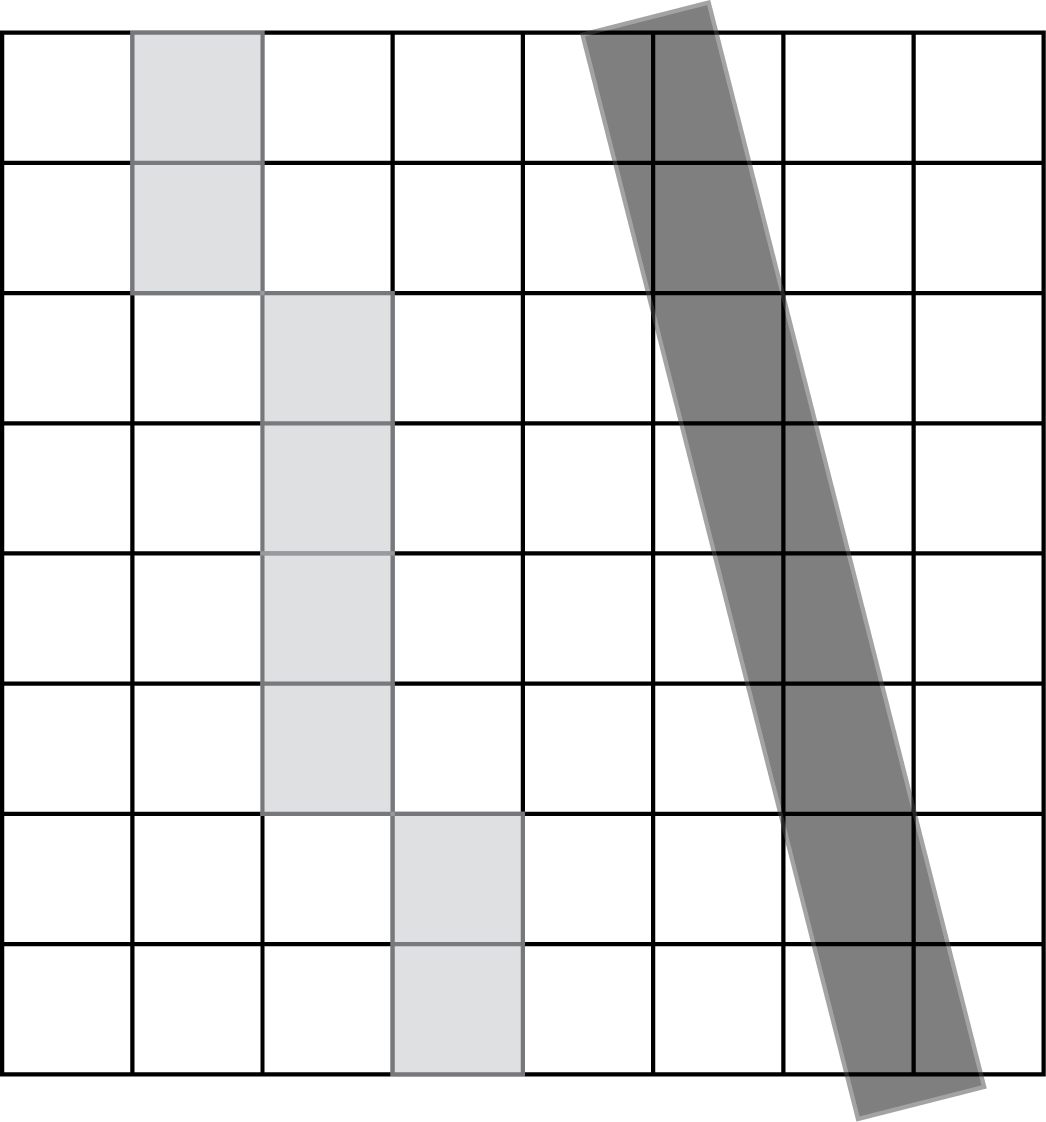
\includegraphics[width=0.55\textwidth]{Dissertation/images/part1_img/ART-Discr-ru}
 \caption{Различия в методе рассчета лучевых сумм}
Слева --- луч в БПХ, справа --- некоторе приближение бесконечно тонкого луча.
\label{fig:hough_radon}
\end{figure}


Обычно итерация алгебраического метода выглядит как шаг в направлении антиградиента минимизируемого функционала ошибки:
\begin{equation}\notag
  \Delta \textbf f = \sum_\varphi {{W^\varphi}^{\mathrm T}(\textbf p - W\textbf f) } = W^{\mathrm T}(\textbf p - W \textbf f).
\end{equation}
где $W$ это оператор преобразования Хафа или томографической проекции.
  
Для асимптотического ускорения итерации алгебраического метода предложено использовать преобразование Хафа, основанное на диадических паттернах --- быстрое преобразование Хафа.
Общая схема алгоритма состоит в следующем: сначала данные эксперимента преобразуются таким образом, чтобы реальные углы и смещения измерительной схемы соответствовали углам и смещениям координат БПХ.
Строки БПХ делятся по четвертям, соответствие строк реальным углам устанавливается соотношениями:
\begin{equation} \notag
\begin{array}{lll}
\alpha^\rom{1}_i &= \pi - & \arctan{\frac{N-1-i}{N-1}} \\
\alpha^\rom{2}_i &= &\arctan{\frac{i - (N-1)}{N-1}} \\
\alpha^\rom{3}_i &= \frac \pi 2 - & \arctan{\frac{3(N-1)-i}{N-1}} \\
\alpha^\rom{4}_i &= \frac \pi 2 - & \arctan{\frac{i - 3(N-1)}{N-1}}
\end{array}
\end{equation}


После этого запускается итеративная процедура, вычисляющая прямую проекцию от текущей гипотезы о восстанавливаемом объекте, производится вычисление невязки, рассчитывается ее градиента, затем гипотеза обновляется.
Приведем описание основных шагов алгоритма.
Изменение модели прямой проекции состоит в изменении геометрических свойст проекционных лучей. 
Если в обычных томографических методах измерения вдоль одного направления вычисляются путем поворота восстанавливаемой функции на определенный угол, и последующего суммирования изображения по строкам, то в новой схеме вычисление угловых прекций осуществляется применением быстрого преобразования Хафа.
При этом, вычисляя невязку, нужно учитывать, что в реальных экспериментальных измерениях не все углы БПХ присутствуют: если число проекционных углов составляет $n_\varphi$, то в координатах пространства БПХ такая картина будет иметь нули по $4 * n - 3 - n_\varphi$ угловым отсчетам, что в случае изображения размера 256х256 и 180 экспериментально измеренных проекциях даст картину преоразования хафа с пустыми 841 из 1021 строк.

Эффективная реализация обратной проекции (вычисления градиента невязки) с помощью БПХ не так тривиальна и ниже дано описание ее вычисления.
БПХ-изображение делится на 4 части по направлениям линий проекции: вертикальные-левые, вертикальные-правые, горизонтальные-левые и горизонтальные-правые.
Соответственно, матрица проекции тоже разделяется на 4 независимые части по строкам $W = \left( W^\rom{1}\ W^\rom{2}\ W^\rom{3}\ W^\rom{4} \right)^{\mathrm T}$.
В главе приведено доказательство того, что для каждой четверти $\xi$ матрицы БПХ имеет место соотношение $W^\xi = {W^\xi}^{\mathrm T}$.
Таким образом, вычисление градиента в значении невязки для одной четверти углов сводится к расчету прямого БПХ от этой невязки.  
Для каждой четверти преобразования Хафа выполняются аналогичные действия и общая невязка получается суммированием невязок по четвертям:

\begin{equation} \notag
W^{\mathrm T}\left( \textbf p - W \textbf f\right) = \sum_{\xi = \rom{1}} ^{\xi = \rom{4}} {W^{\xi} \left(\textbf p - W \textbf f \right)^{\xi}}
\end{equation}

Итерации продолжаются пока не достигнут критерий останова по количеству итераций либо по значению невязки.
Данный метод рассчета прямой и обратной проекции использует шаг по всем кординатам градиента, поэтому больше похож на метод SIRT.
При этом одна минимально необходимо обновлять лишь четверть проекционных углов за раз, поэтому возможно приблизить способ обновления гипотезы к методу SART, который обладает лучшей сходимостью решения.
Из-за использования БПХ для расчета проекций, метод получил название FHT-SIRT.
В главе показано, что можно использовать метод FHT-SIRT для восстановления томографии, что подтверждается численными экспериментами на симулированных и реальных экспериментальных измерениях.
Использование FHT-SIRT позволяет снизить асимптотическую сложность одной итерации метода с $O(n^2 * n_\varphi) \approx O(n^3)$ до $O(n^2 \log n)$.
При восстановлении данных реальных экспериментов количество и значения проекционных углов сильно меньше чем предусмотрено в БПХ. 
Поэтому в главе так же исследовано влияние ``степени разрежения'' (т.е. доли пустых строчек в БПХ) на качество сходимости \ref{fig:conv_all} a).

\begin{figure}
\centering
\begin{tabular}{@{}c@{}c}
    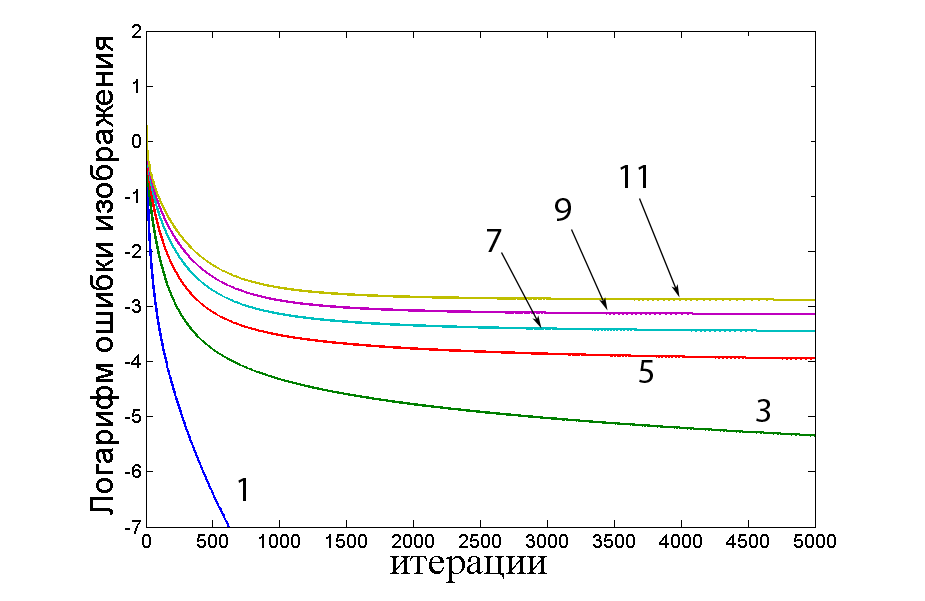
\includegraphics[width=0.50\textwidth]{Dissertation/images/part1_img/raw}
&
    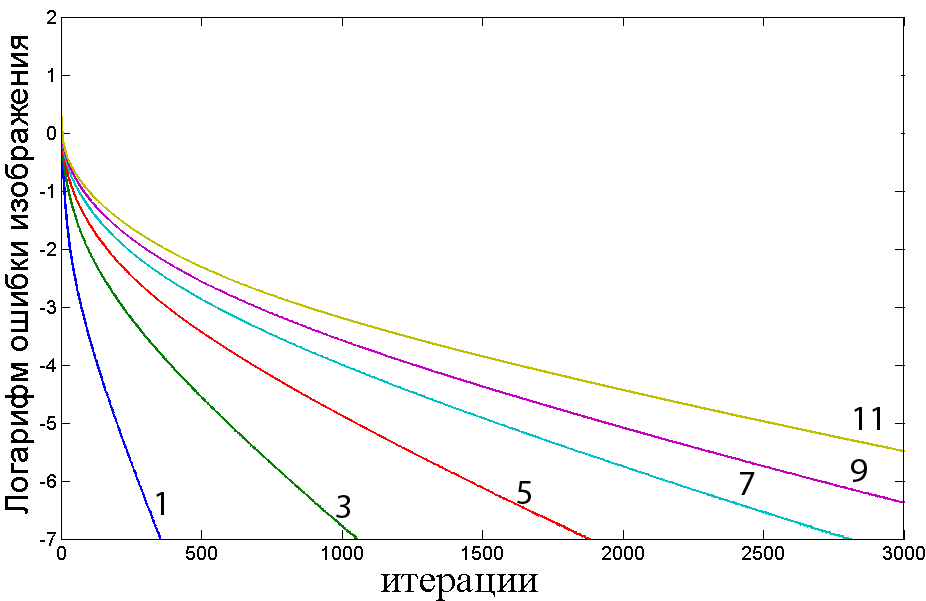
\includegraphics[width=0.50\textwidth]{Dissertation/images/part1_img/medk}
\\
   \small a) & \small b)
\end{tabular}
  \caption{Зависимость среднеквадратичной ошибки изображения от числа итераций.}
Номер графика соответствует степени разрежения. а --- Без регуляризации, б --- Медианный фильтр в качестве регуляризации.
\label{fig:conv_all}
\end{figure}

\vspace{2cm}

Еще одно преобразование, которое применяется к данным при переводе измеренных проекций из координат геометрии измерений $\rho, \varphi$ в координаты пространства БПХ, --- это учет изменения ширины БПХ-луча в зависимости от угла наклона, --- нормировка значений в строке по ширине и интенсивности:
\begin{enumerate}[label=\Roman*.]
	\item растяжение в $\frac 1 {\cos \alpha_i}$ раз
	\item растяжение в $\frac 1 {\cos \alpha_i}$ раз
	\item растяжение в $\frac 1 {\sin \alpha_i}$ раз
	\item растяжение в $\frac 1 {\sin \alpha_i}$ раз
\end{enumerate}

Чтобы повысить сходимость метода исследуются возможные регуляризации при применении метода FHT-SIRT.
Исследуются регуляризация с применением медианного, билатерального фильтров после каждой итерации, а так же регуляризация по Тихонову.
В последней части главы приводятся результаты восстановления с применением указанных видов регуляризации.
В частности, сравнение сходимости реконструкции без регуляризации и при использовании медианного фильтра приведено на рис. \ref{fig:conv_all} б).

\vspace{5mm}

В \underline{\textbf{третьей главе}} приведено описание предложенной модели формирования проекций при наличии в объекте сильнопоглощающих включений.
При прохождении через такие включения, например, металлический протез в зубе, большая часть зондирующего излучения поглощается.
В результате количество фотонов, достигающих детектора, недостаточно для активации его пикселя.
С таких пикселей считывается значение 0, хотя, на самом деле, можно лишь сказать, что значение, считанное с этих пикселей находится где-то в интервале $[0, \delta_{min})$, где $\delta_{min}$ --- минимальный порог срабатывания детектора, или уровень шума.
Восстановление без учета ошибок, содержащихся в синограмме, приведет к возникновению артефактов на восстановленном изображении (рис. \ref{im:quadprog}b,c). 

Для того, чтобы избежать появления этих артефактов, задачу восстановления в алгебраическом подходе можно модифицировать, вводя ограничения типа неравенства для пикселей, значение которых 0 (или $<  \delta_{min}$).
Для прологарифмированных значений, условие $I < \delta_{min}$ переходит в условие $p > \ln\frac{I_0}{\delta_{min}} = \delta$.
Тогда, с учетом перехода к логарифмам измеренной интенсивности, алгебраическая постановка задачи восстановления переходит в задачу условной оптимизации 

\begin{equation} \notag
  \label{eq:quadprog_ineq}
  \begin{cases}
  \Norm{P^{\textup{изм.}} - W(f)} \rightarrow \min\limits_f & w.r.t \\
  \sum_i f_{i} \omega_{ij} = P_j, & \mbox{если } P^{\textup{изм.}}_j < \delta \\
  \sum_i f_{i} \omega_{ij} > \delta, & \mbox{если } P^{\textup{изм.}}_j = \delta
  \end{cases}
\end{equation}

Так как функционал ошибки квадратичный, а ограничения - линейные, для решения этой минимизационной задачи эффективным будет применить метод квадратичного программирования.
При этом в формулировке оптимизационной задачи присутствует полная матрица преобразования Хафа $\omega_{ij}$.
Для размера восстанавливаемого изображения 256х256 и 180 проекционных углов при использовании типа данных float64 такая матрица будет занимать порядка 32Гб.
Общая формула для расчета размера матрицы это $\sqrt{2} * n * n_\varphi \times n * n$.
При этом ненулевые значения для каждого столбца находятся только в $\approx n$ ячейках, делая возможным использование инструментария для работы с разреженными матрициы.

Результаты востановления методом квадратичного программирования представлены на рис. \ref{im:quadprog}.
Результаты представлены на небольшом фантоме размера 10х10 пикселей и 35 проекционных углов.

\begin{figure}
  \centering
  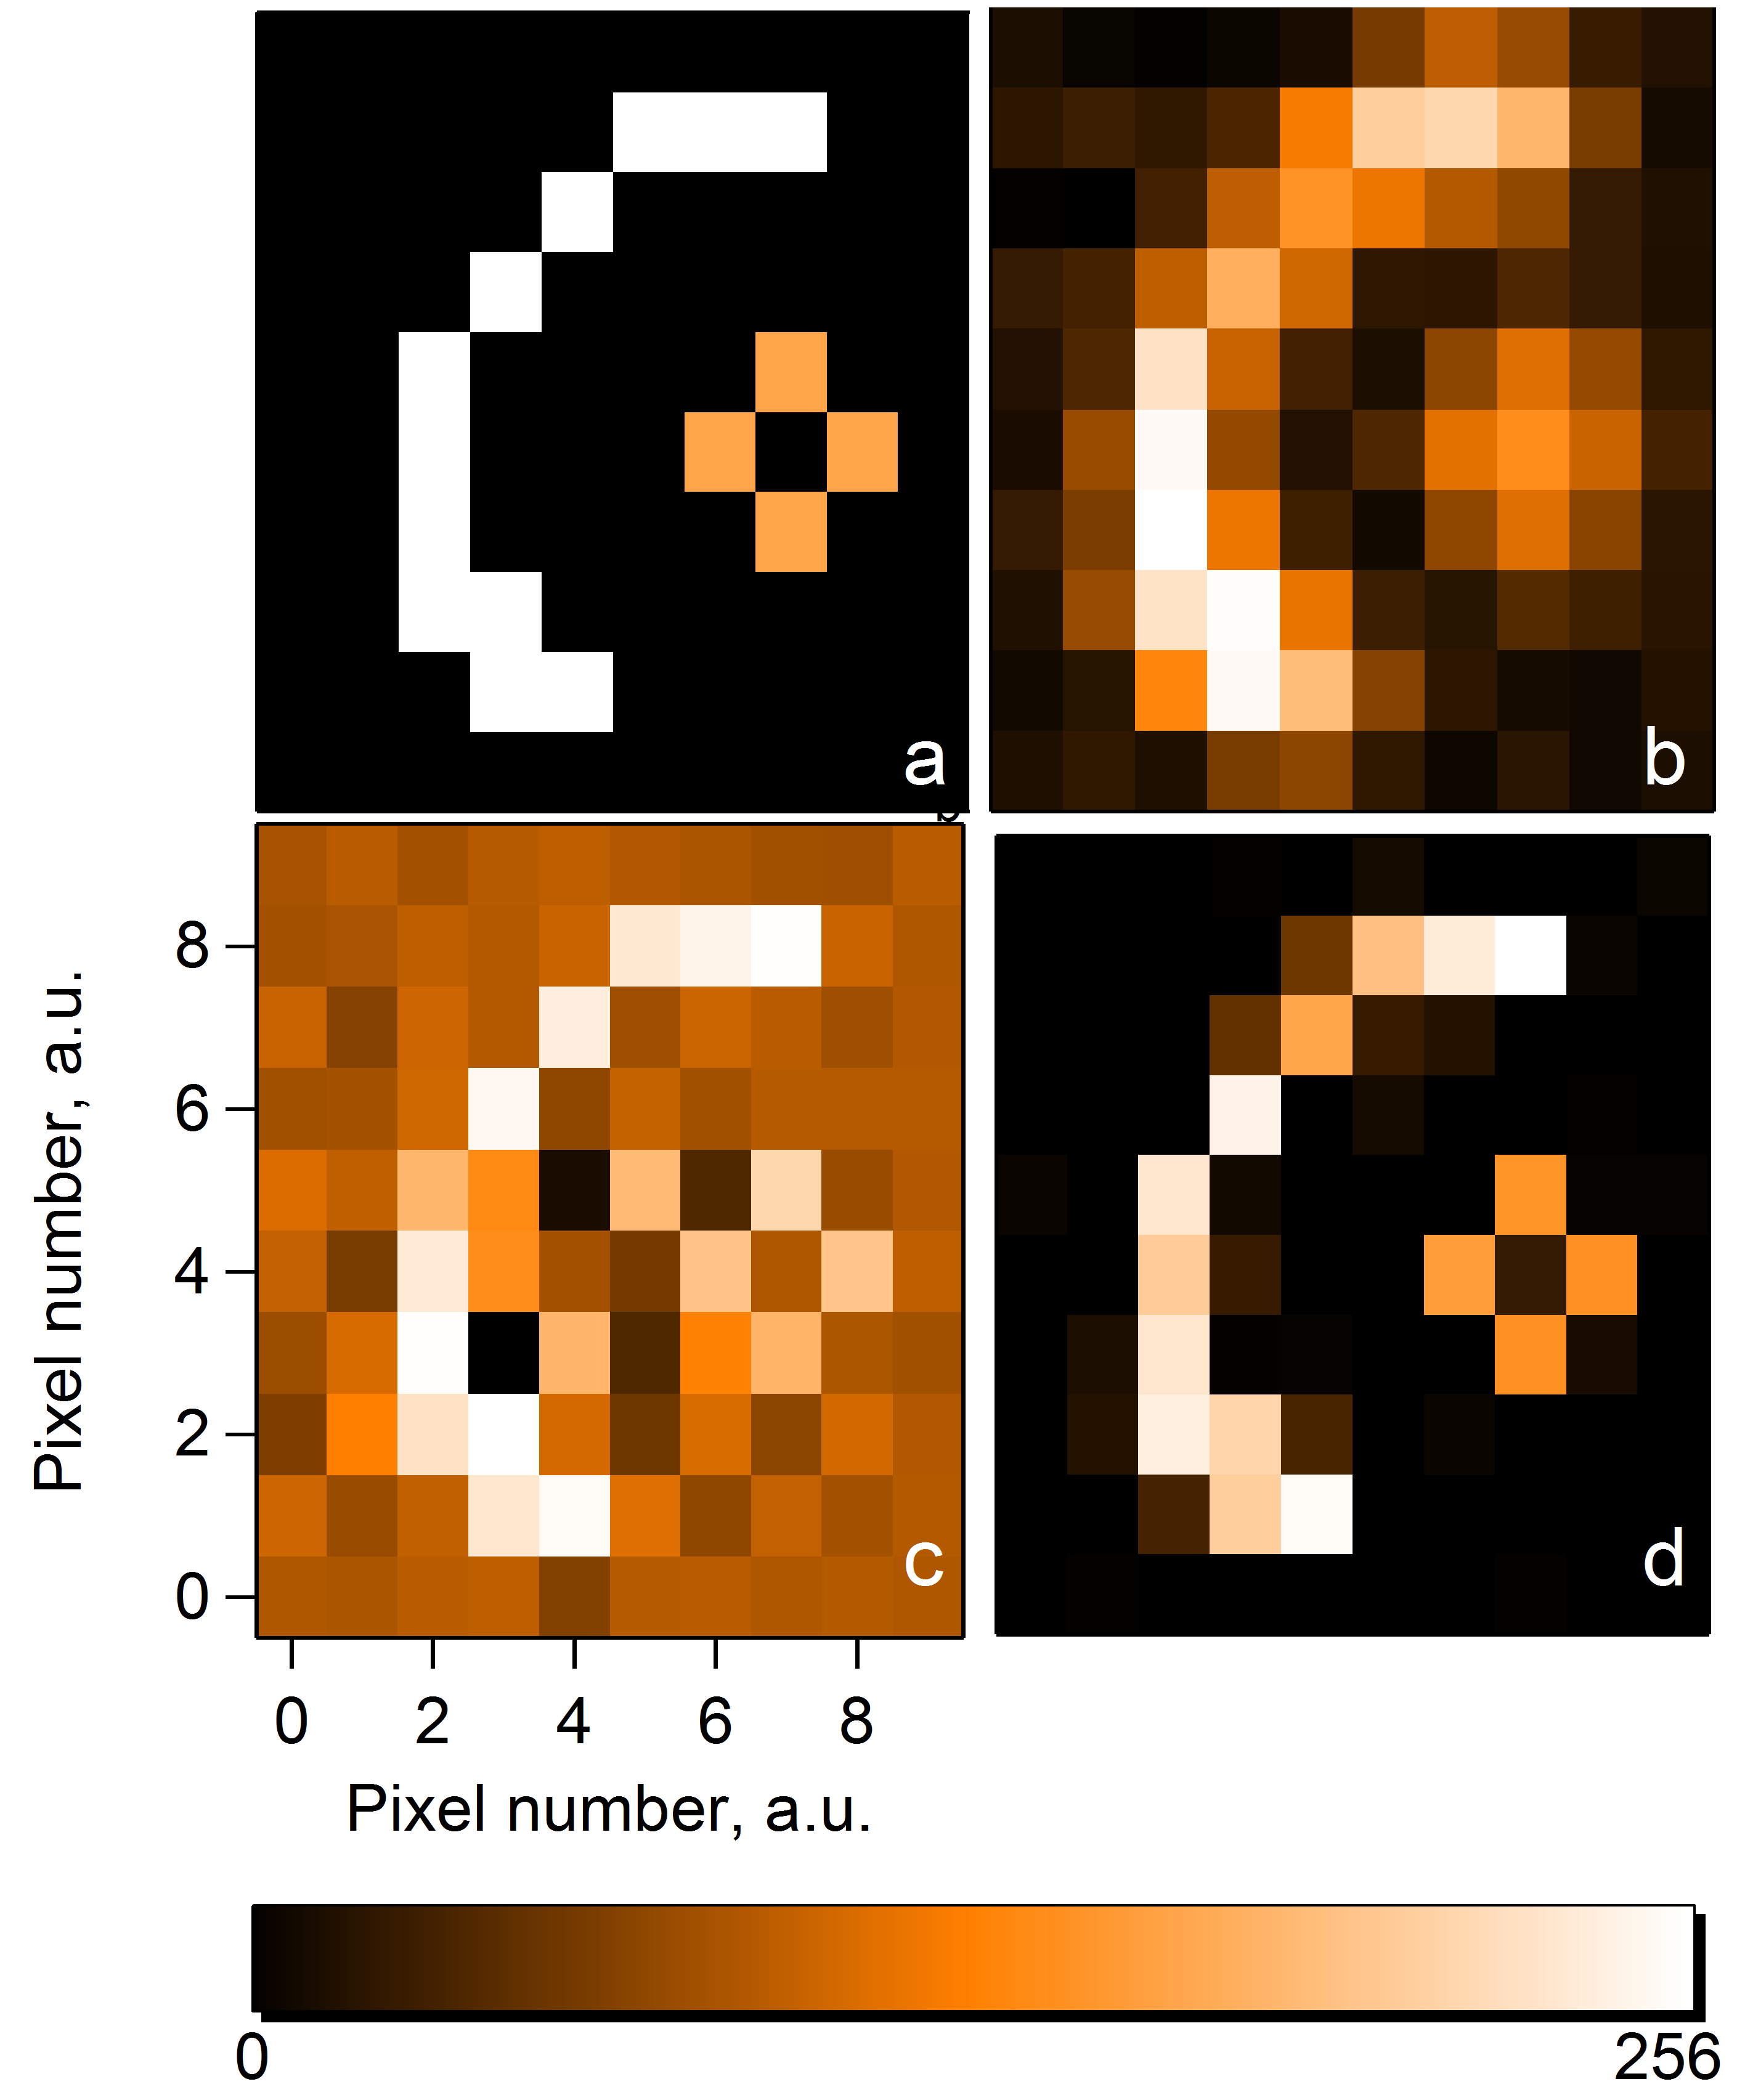
\includegraphics[width=0.8\textwidth]{Dissertation/images/part2_img/quadprog}
  \caption{Слева-направо сверху-вниз: a) - фантом, использованный для расчета лучевых сумм. b)- результат восстановления методом FBP. c) - результат восстановления методом квадратичного программирования без ограничений-неравенств. d) - результат восстановления методом квадратичного программированиея с учетом ограничений-неравенств (предложенный метод)}
  \label{im:quadprog}
\end{figure}

Использование жестких ограничений не всегда стабильно отностильно наличия шумов в данных.
Этот подход так же требует работы с матрицей проекции, которая даже в разреженном виде требует больших вычислительных ресурсов.
Этого можно избежать, если заменить уравнения ограничений задачи оптимизации на аддитивные квадратичные регуляризирующие штрафы, выражающие эти ограничения.
Такой подход называется методом мягких ограничений.
В контексте решаемой задачи и ее ограничений, предлагается ввести квадратичные штрафы за нарушение выхода за границы порога $\delta$.
Если ввести диагональные матрицы-индикаторы нарушения ограничений, $J_{ii} = \left\{1, \mbox{если} \left(\sum f_{i} \omega_{ij} \geq \delta \right), \mbox{иначе } 0\right\}$, и $K = E - J$, то задача минимизации с мягкими ограничениями будет выглядеть как

\begin{equation} \notag
  \label{eq:soft-ineq}
  ||K(Wf - P^{\textup{изм}})||^2 + \alpha ||J(Wf - \delta)||^2 \to \min\limits_f,
\end{equation}

В работе проводится исследования метода мягких ограничений с использованием данных лабораторных измерений.
Измерения проводились на прототипе программно-аппаратного томографического комплекса созданного и функционирующего в лаборатории рефлектометрии и малоуглового рассеяния ФНИЦ ``Кристаллография и фотоника'' РАН.
Восстановления фантомов, а так же реального образца, можно наблюдать на рисунках.
В работе производится сравнение восстановления методами мягких ограничений и метода квадратичного программирования.

\begin{figure}
  \centering
  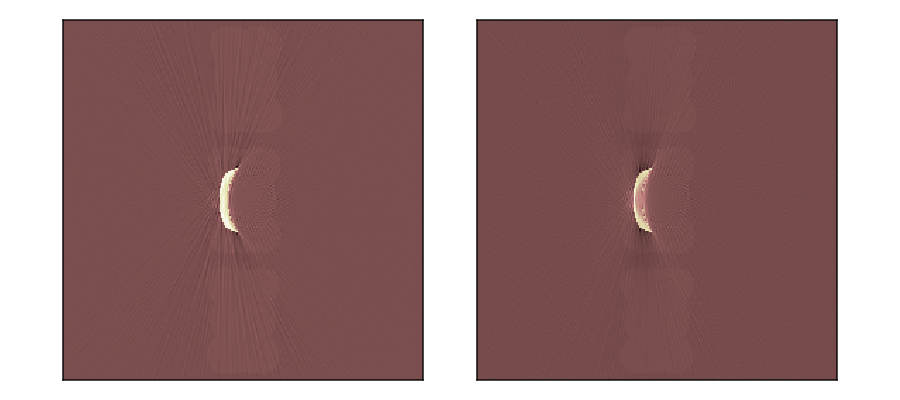
\includegraphics[width=0.9\textwidth]{Dissertation/images/part2_img/sample}
  \caption{Реконструкции методом мягких ограничений.}
  \label{fig:sample}
\end{figure}

\vspace{10mm}

На рис. \ref{fig:sample} представлены результаты реконструкции фантома, моделирующего золотое (Au) включение в зубе (Ca).
Результаты восстановления методом мягких ограничений (слева) и методом, в которых данные выше порога просто игнорируются (справа), 200 итераций алгебраического метода, коэффициент регуляризациии --- 30.

\begin{figure}
\centering
\begin{tabular}{@{}c@{}c}
    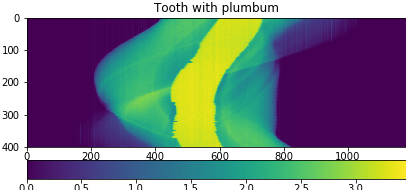
\includegraphics[width=0.50\textwidth]{Dissertation/images/part2_img/tooth_sino}
&
    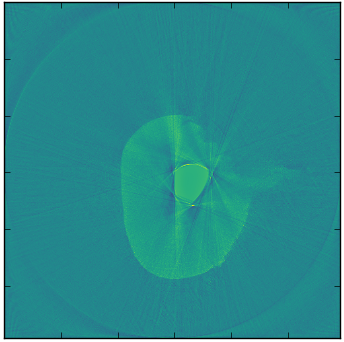
\includegraphics[width=0.50\textwidth]{Dissertation/images/part2_img/soft_ineq_pb_tooth}
\\
   \small a) & \small b)
\end{tabular}
  \caption{a --- Синограмма молочного зуба с включением из свинца. б --- результат восстановления методом мягких ограничений}
\label{fig:tooth_sino_rec}
\end{figure}

В качестве реального образца была взята синограмма зуба со свинцовым включением.
В качестве порога было выбрано значение 2.9, соответствующее последнему пику интенсивности на гистограмме синограммы.
Обоснование выбора этого значения проиллюстрировано на гистограмме на риc. \ref{fig:pb_hist}.


\begin{figure}
  \centering
  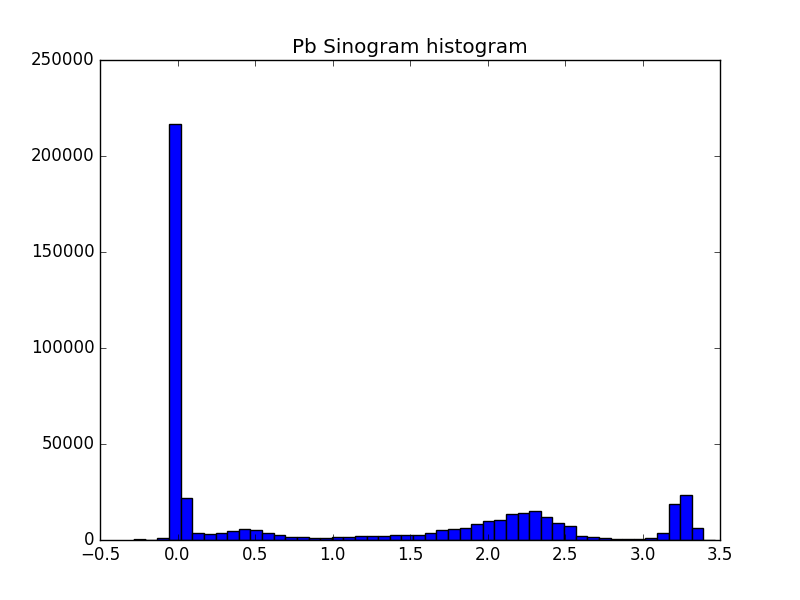
\includegraphics[width=0.9\textwidth]{Dissertation/images/part2_img/pb_hist}
  \caption{Распределение интенсивностей синограммы}
  \label{fig:pb_hist}
\end{figure}



\vspace{5mm}

В \underline{\textbf{четвертой главе}} описан предложенный подход для восстановления томографических измерений при зондировании полихоматическим илучением, основанный на использовании алгебраического метода реконструкции.
В большом количестве экспериментальных схем спектр источника является полихроматическим, то есть энергия источника имеет нетривиальный несингулярный спектр.
Использование монохроматора, с одной стороны, позволяет понизить сложность задачи реконструкции, сведя решение к монохроматическому случаю, но это увеличивает время получения набора томографических проекций, с другой стороны.
Это делает метод неприменимым для практической медицины и промашленной интроскопии.
Свойства поглощения материала меняются в зависимости от частоты зондирующего излучения.
В результате, реальная измеренная детектором интенсивность рентгеновского излучения не соответствует модели, используемой в традиционных подходах к восстановлению.
Это значит, что заложенные в алгоритме реконструкции модели прямой и обратной проекции либо будут неспособны обеспечить сходимость оптимизационной процедуры, либо сойдутся к ложному минимуму, не являющемуся в реальности решением физической задачи.
В обоих случаях восстановление традиционными алгоритмами синограммы, снятой при зондировании немонохроматическим излучением, повлечет появление артефактов на восстановленном изображении.

В данной главе рассматривается метод, позволяющий учесть спектральные особенности взаимодействия материалов объекта с излучением.
При этом предлагается перейти от восстановления распределения линейного коэффициента ослабления излучения к восстановлению пространственного распределения концентраций элементов $c_k(x,y)$, массовые коэффициенты ослабления которых затабулированы:

\begin{equation} \notag
  \label{eq:white_fp_final}
  I(c)_j = \int_0^{+\infty} {d\lambda \left\{
    I_0(\lambda) \exp{\left(
      -\sum_{k=1}^K {\rho \kappa_k(\lambda) (W c_k)_j} 
      \right)}
  \right\}}
\end{equation}

,здесь за $\kappa_k(\lambda)$ обозначен массовый коэффициент поглощения вещества $k$ на длине волны $\lambda$, а $I_0(\lambda)$ --- спектр источника, $\rho$ --- линейный размер пикселя, индекс $j$ обозначает номер пикселя на изображении измеренных проекций.
Следуя алгебраическому подходу, реконструкция проводится с помощью градиентного спуска оптимизации квадратичной функции потерь 
$
Q(c) = \frac {\left(I(c) - t\right)^2} {S}
$
, где $t$ --- измеренные интенсивности прошедшего через объект излучения, 
$S = \int_0^{+\infty} { I_0(\lambda) d\lambda}$
 --- суммарная интенсивность зондирующего излучения.

Общий вид итерации восстановления будет иметь вид

\begin{equation} \notag
\label{eq:part3_whitegrad}
  \nabla_k \ Q = 2W^\intercal R_k \text{, где } R_{kj} = \frac {(I(c) - t)_j} {S} \mu_{kj}
\end{equation}
, а формулы для вычисления весов невязок по каждому элементу приведены ниже:
\begin{equation} \notag
  \label{eq:weights}
  \mu_{k} = \int_0^{+\infty} {d\lambda \left\{
    -\rho \kappa_k(\lambda) 
    I_0(\lambda)
    \exp{\left(
      -\sum_{s=1}^K {\rho \kappa_s(\lambda) (W c_s)} 
         \right)}
    \right\}}
\end{equation}

В указанной итерационной схеме отсутсвует пространственные различия в формулах обновления концентраций разных элементов. 
Поэтому необходимо вводить дополнительную регуляризацию.
Предлагаемое решение состоит в том, чтобы запретить находиться в одной пространственной ячейке одновременно разным материалам $c_{k_1} \odot c_{k_2} = 0, \mbox{если } k_1 \neq k_2$, что при применении метода мягких ограничений выглядит как аддитивный регуляризующий член 
\begin{equation} \notag
	\sum_{k_1 != k_2} {||c_{k_1} \odot c_{k_2}||^2}
\end{equation}

Здесь за $c_{k_1} \odot c_{k_2}$ обозначена поэлементная операция умножения массивов.

\begin{comment}
На рисунке \ref{fig:whiteres} представлены результаты восстановления для фантома с использованием и без использования регуляризации.
На верхнем ряду представлены распределения концентраций каждого элемента в первых двух столбцах, а в третьем - их отношение.
Наблюдать отношение концентраций разных элементов полезно для контроля пространственного разделения их характеристик.
В случае, если оптимизация вырождается по координате элементов, третий столбец будет равномерно одинакового значения.
Снизу представлены аналогично преобразования Хафа для концентраций элементов и их отношения в третьем столбце.

\begin{figure}
\label{fig:whiteres}
\centering
\begin{tabular}{@{}c@{}c}
  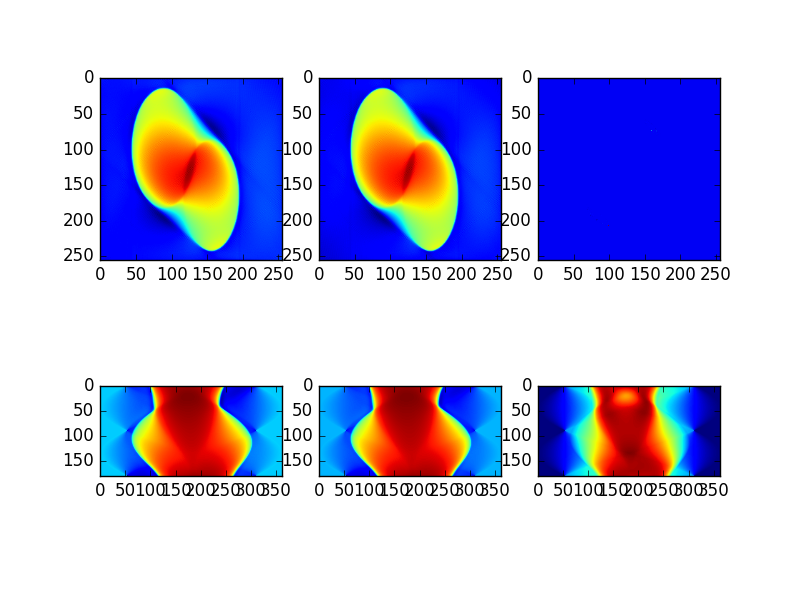
\includegraphics[width=0.5\textwidth]{Dissertation/images/part3_img/no_reg_iteration_25} &
  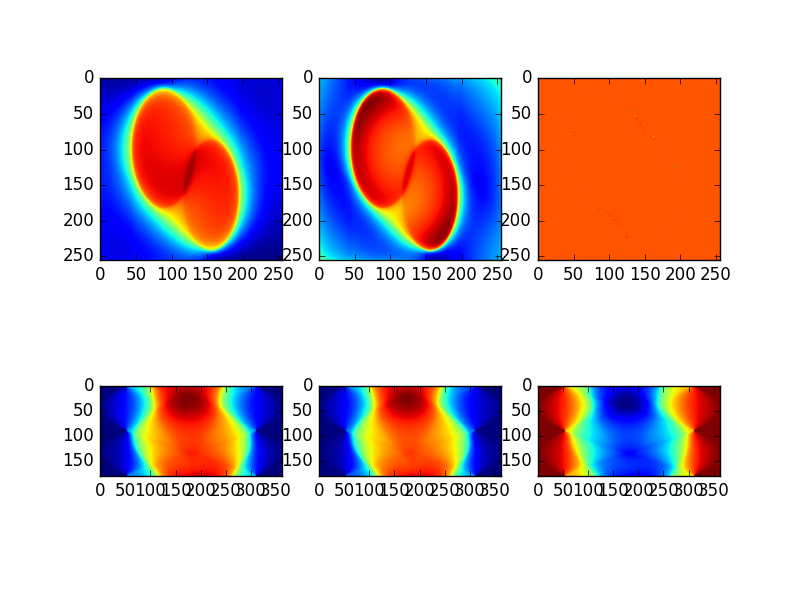
\includegraphics[width=0.5\textwidth]{Dissertation/images/part3_img/mul_reg_iteration_150}
  \\
  а) &
  б) \\
\end{tabular}
\caption{Восстановление с помощью МВН. а) без регуляризации. б) мультипликативная регуляризация}
\vspace{5mm}
\end{figure}
\end{comment}

На рисунке \ref{fig:whiteres} представлен результат реконструкции фантома, состоящего из трех сильнопоглощающих включений в окружении из слабопоглощающего фона.
Алгоритму взвешанных невязок с мультипликативной регуляризацией удалось выделить элементы включения на отдельном канале концентраций.
Таким образом, показана применимость выбранной модели для реконструкции концентраций смеси в условиях полихроматического зондирования.

\begin{figure}
\label{fig:whiteres}
\centering
  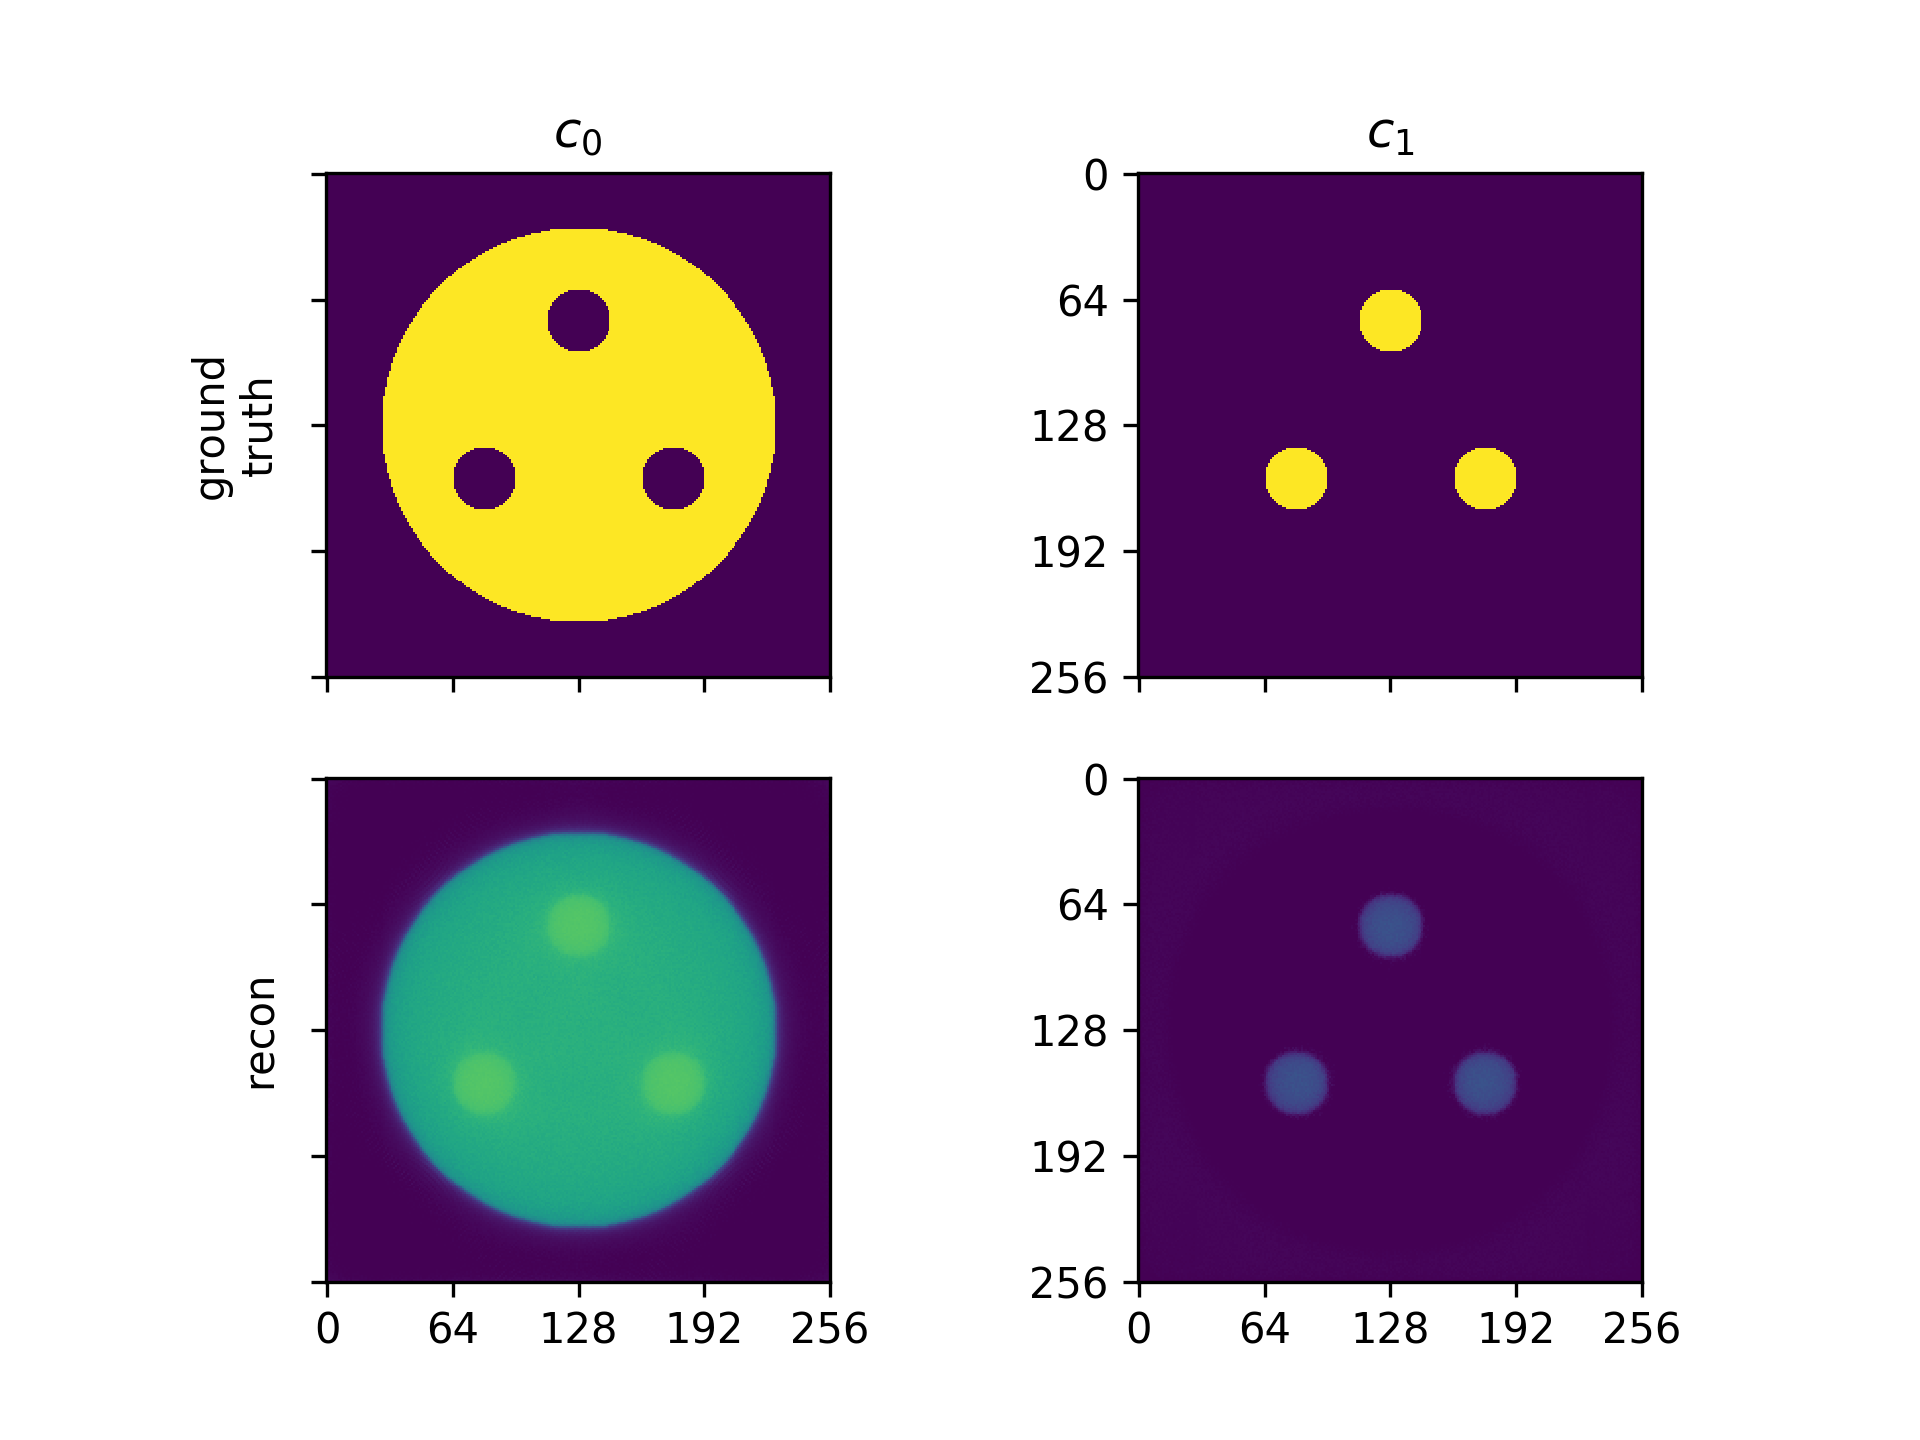
\includegraphics[width=0.9\textwidth]{Dissertation/images/part3_img/recon} 
\caption{Восстановление с помощью МВН. Верхний ряд: исходные данные, использованные для моделирования. Нижний ряд: восстановленные концентрации элементов.}
\vspace{5mm}
\end{figure}

Как видно из рисунков, мультипликативная регуляризация позволяет пространственно разделить концентрации различных элементов.

В \underline{\textbf{заключении}} приведены основные результаты работы, которые заключаются в следующем:
%% Согласно ГОСТ Р 7.0.11-2011:
%% 5.3.3 В заключении диссертации излагают итоги выполненного исследования, рекомендации, перспективы дальнейшей разработки темы.
%% 9.2.3 В заключении автореферата диссертации излагают итоги данного исследования, рекомендации и перспективы дальнейшей разработки темы.
\begin{enumerate}
  \item Получено аналитическое выражение для операции транспонированного быстрого преобразования Хафа. Доказана теорема о симметричности четверти БПХ, отвечающей одной группе ориентаций лучей. Получен метод вычислительно эффективного вычисления транспонированного преобразования.
  \item Построен вычислительно эффективный алгебраический метод восстановления измерений компьютерной томографии на основе БПХ. Произведена адаптация метода для работы с данными реальных измерений. Изучены свойства пространства БПХ, влияние различной регуляризации на процесс восстановления.
  \item Построен метод восстановления рентгеновской томографии методом квадратичного программирования для объектов, содержащих сильнопоглощающие включения. На реальных экспериментальных измерениях проведено исследование метода мягких ограничений \todo{и сравнение с методом квадратичного программирования}
  \item Построен алгебраический алгоритм восстановления томографии в задаче зондирования полихроматическим излучением, основанный на вычиследнии взвешанных невязок по каждому из элементов, входящих в состав исследуемого образца. Предложены варианты регуляризации для востановления в полихроматической моде. \todo{описать, какой получен результат}
\end{enumerate}


\begin{comment}
%\newpage
При использовании пакета \verb!biblatex! список публикаций автора по теме
диссертации формируется в разделе <<\publications>>\ файла
\verb!../common/characteristic.tex!  при помощи команды \verb!\nocite! 
\end{comment}

\newpage
\ifdefmacro{\microtypesetup}{\microtypesetup{protrusion=false}}{} % не рекомендуется применять пакет микротипографики к автоматически генерируемому списку литературы
\ifnumequal{\value{bibliosel}}{0}{% Встроенная реализация с загрузкой файла через движок bibtex8
  \renewcommand{\bibname}{\large \authorbibtitle}
  \nocite{*}
  \insertbiblioauthor           % Подключаем Bib-базы
  %\insertbiblioother   % !!! bibtex не умеет работать с несколькими библиографиями !!!
}{% Реализация пакетом biblatex через движок biber
  \ifnumgreater{\value{usefootcite}}{0}{
%  \nocite{*} % Невидимая цитата всех работ, позволит вывести все работы автора
  \insertbiblioauthorcited      % Вывод процитированных в автореферате работ автора
  }{
  \insertbiblioauthor           % Вывод всех работ автора
%  \insertbiblioauthorgrouped    % Вывод всех работ автора, сгруппированных по источникам
%  \insertbiblioauthorimportant  % Вывод наиболее значимых работ автора (определяется в файле characteristic во второй section)
  % \insertbiblioother            % Вывод списка литературы, на которую ссылались в тексте автореферата
  }
}
\ifdefmacro{\microtypesetup}{\microtypesetup{protrusion=true}}{}

